\documentclass[a4paper,12pt]{report}
\usepackage{color}
\usepackage{hyperref}
\hypersetup{
    colorlinks,
    citecolor=black,
    filecolor=black,
    linkcolor=black,
    urlcolor=black
}
\setcounter{secnumdepth}{0}
\usepackage{graphicx}
\usepackage{epstopdf}
\epstopdfsetup{outdir=./}
\usepackage{amsmath}
\usepackage[table,xcdraw]{xcolor}
\usepackage{amssymb}
\usepackage{listings}
\definecolor{anti-flashwhite}{rgb}{0.95, 0.95, 0.96}
\lstset{
	language=C++,
    basicstyle=\ttfamily,
    keywordstyle=\color{blue}\ttfamily,
    stringstyle=\color{red}\ttfamily,
	commentstyle=\color{green}\ttfamily,
    morecomment=[l][\color{magenta}]{\#},
    backgroundcolor=\color{anti-flashwhite}
}
\begin{document}
\title{
\textbf{CS5300 - Parallel \& Concurrent Programming}\\~\\
\begin{large}
\textbf{Comparing Different Parallel Implementations for Identifying Prime Numbers}\\
\end{large}
\begin{large}
\textbf{Assignment Report}
\end{large}
}
\author{\textbf{Sagar Jain - CS17BTECH11034}\\}
\maketitle
\begin{large}
\tableofcontents
\end{large}
\newpage
\section{Program Design}
The program calls the three algorithms DAM, SAM1 \& SAM2, sequentially and records the time taken for each of them. Elements common to all the three algorithms are:
\begin{itemize}
\item \texttt{pthreads} have been used for multithreading.
\item \texttt{chrono} had been used to record time.
\item Conditional compilation has been used for writing to output files to avoid taking printing time into consideration when calculating the time taken for the algorithms.
\item The same method (\texttt{isPrime}) has been used to check primality for all the algorithms to ensure the differences in times are purely based on the load distribution.
\item The \texttt{isPrime} function uses a precomputed list of all the primes till $\;\sqrt[]{n}$ and for any given input \texttt{k} checks if there is any prime less than \texttt{k} in the list which divides it.
\end{itemize}
\subsection{Dynamic Allocation Method}
The following is the description of the DAM algorithm:
\begin{itemize}
\item The method for the DAM algorithm is \texttt{dam}.
\item This method creates and launches \texttt{M} threads which execute the \texttt{dam\_thread} method.
\item The \texttt{dam\_thread} method uses the \texttt{getAndIncrement} method for an instance of the \texttt{Counter} class to be allocated numbers to check for primality.
\item Based on the test it either writes to the output file or continues looping until finally being allocated a value greater than $10^{N}$.
\item The \texttt{Counter} class uses a \texttt{mutex} lock to make the \texttt{getAndIncrement} function mutually exclusive.
\end{itemize}
\subsection{Static Allocation Method I}
\begin{itemize}
\item The method for the SAM I algorithm is \texttt{sam1}.
\item This method creates and launches \texttt{M} threads and gives an index to each one of them between \texttt{1} to \texttt{M}. These threads execute the method \texttt{sam1\_thread}.
\item The \texttt{sam1\_thread} simply checks the primality of all the numbers \\$M*i + index \; \forall i \; \in [0, N/M]$. Here, \texttt{index} is allocated to threads when they are launched.
\end{itemize}
\subsection{Static Allocation Method II}
\begin{itemize}
\item The method for the SAM II algorithm is \texttt{sam2}.
\item This method creates and launches \texttt{M} threads and gives an index to each one of them between \texttt{1} to \texttt{M}. These threads execute the method \texttt{sam2\_thread}.
\item To avoid checking for even numbers, the optimisations used here is that we distribute the odd numbers evenly among the threads. To do this we use the same loop as in \texttt{SAM I} but instead of checking the primality of the $M*i + index$ we check for the primality of $2*(M*i + index)-1$. In simple words, in \texttt{SAM I} we were checking for the primality of the $i^{th}$ number and in \texttt{SAM II} we are checking for the primality of the $i^{th}$ odd number.
\item \textbf{Point to Note}: The distribution of odd numbers between the threads is fair. Since we use the index to choose the odd numbers, we ensure that every thread gets only one odd number between the $M*i^{th}$ odd number and $M*(i+1)^{th}$ odd number.
\end{itemize}
\newpage
\section{Results \& Graphs}
\subsection{Time Taken vs Value of N}
\begin{center}
\begin{large}
\end{large}
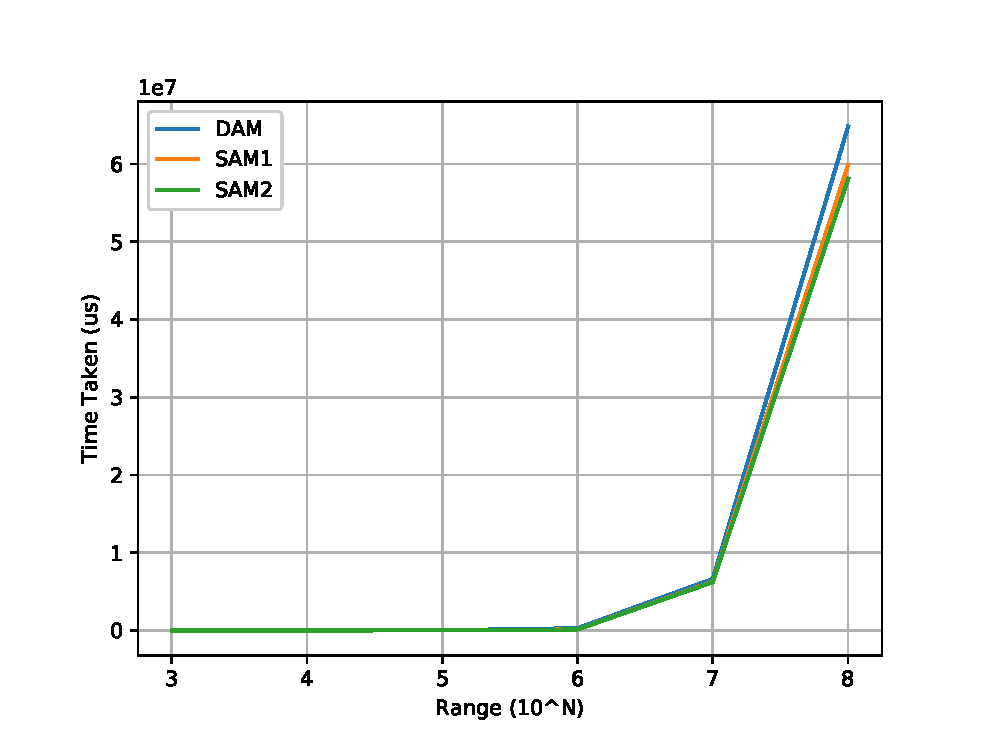
\includegraphics[scale=0.7]{./constantM.eps}
\end{center}
\subsubsection{Inference}
\begin{itemize}
\item Since the x axis of the graph is in logarithmic scale we cannot appreciate the difference in the curves for the lower values of N.
\item We expect \texttt{DAM} to take the longest time since dynamically allocating numbers requires the threads to wait for aquiring the locks. \texttt{SAM II} uses the optimsation of ignoring the even numbers so it is expected to perform better than \texttt{SAM I}. 
\item For values 3, 4, 5 the time taken by \texttt{DAM} was 2 to 3 times that of \texttt{SAM I} which was 1.5 to 2 times \texttt{SAM II}.
\item As the value of N increases, we see that the relation of time taken by \texttt{DAM > SAM I > SAM II} is still according to expectation.
\item Asymptotically, the complexity of all the three algorithms is the same so it is not surprising that for large values of N, the time taken is in the same order of magnitude.
\end{itemize}
\newpage
\subsection{Time Taken vs Number Of Threads}
\begin{center}
\begin{large}
\end{large}
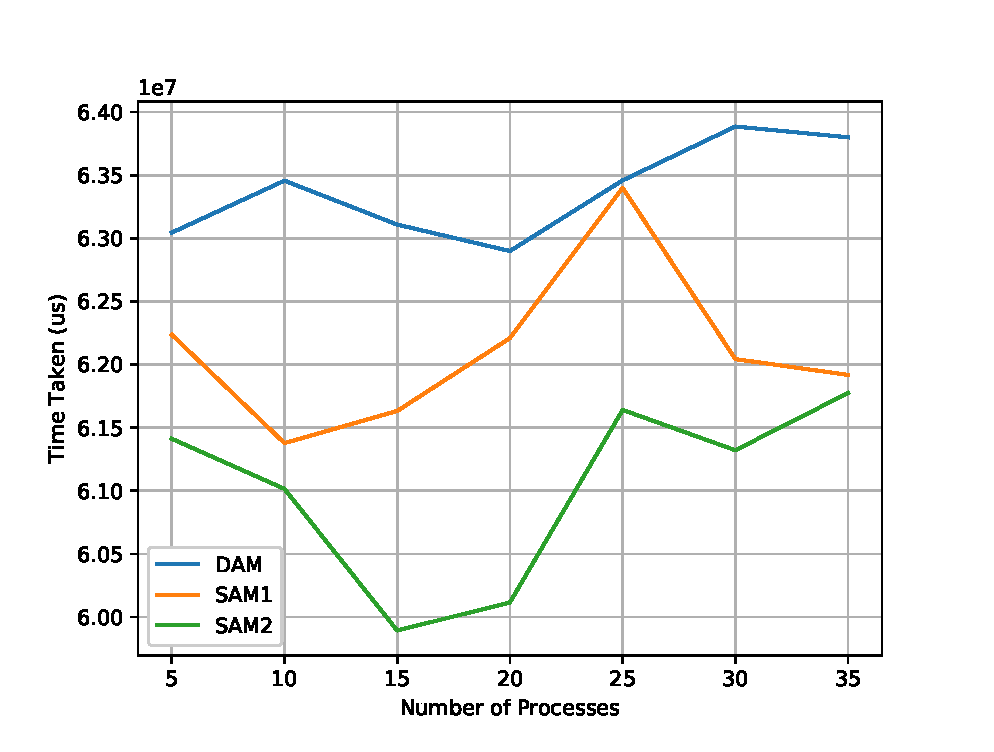
\includegraphics[scale=0.7]{./constantN.eps}
\end{center}
\subsubsection{Inference}
\begin{itemize}
\item This graph would be differ based on the system where the code was run, since increasing the number of threads is only beneficial until the number of threads launched is $<$ number of hardware threads available.
\item Firstly we can see that we still have \texttt{DAM > SAM I > SAM II}. This is as expected.
\item We also notice that the graphs of all the three algorithms have a \textit{U} shape. Which essentially tells that initially increasing the number of threads led to lower time taken but not on increasing beyong 15.
\item The above observation can be explained by the fact that I have an 8 core system with 2 threads in each core, which makes it a total of 16 hardware threads. So before we hit 16 threads we notice improvement in the time taken when increasing the number of threads. But after that increasing the number of threads would lead to more number of context switches on the same physical thread this would lead to more time taken and can be seen in the graph.
\end{itemize}
\newpage

\end{document}